
\documentclass[a4paper  ]{article}
\usepackage{tikz}
\usepackage{pgfplots}
\usetikzlibrary{positioning}
\usetikzlibrary{fit}
\usetikzlibrary{backgrounds}
\usetikzlibrary{calc}
\usetikzlibrary{shapes}
\usetikzlibrary{mindmap}
\usetikzlibrary{decorations.text}

\begin{document}

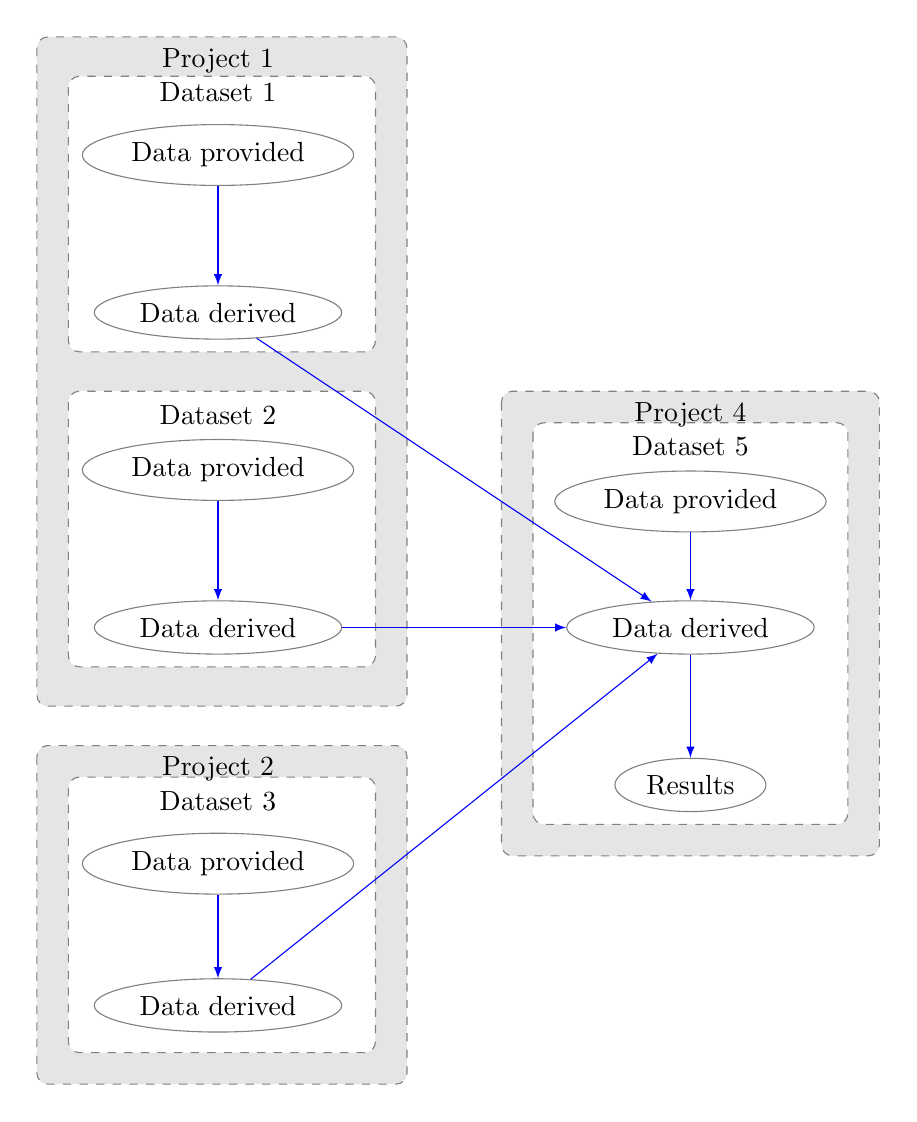
\begin{tikzpicture} [
            outpt/.style={->,blue!80!black,very thick},
            >=stealth,
         every node/.append style={align=center}]
%\tikzstyle{every node}=[draw,rectangle] 

%P1
\node (p1) at (0,1.2){Project 1};
\begin{pgfonlayer}{background}
   % Left-top corner of the background rectangle
   \path (-2.3,1.5) node (a13) {};
   % Right-bottom corner of the background rectanle
   \path (2.4, -7) node (c13) {};
   % Draw the background
   \path[fill=gray!20, rounded corners, draw=black!50, dashed]
   (a13) rectangle (c13);
\end{pgfonlayer}

%D1
\node (d1) at (0,.8) {Dataset 1};
\node (root) at (0,0) [draw=black!50,ellipse] {Data provided};
\node (GH) at (0,-2) [draw=black!50,ellipse]{Data derived}; 
\draw [-latex,color=blue] (root) -- (GH);
\begin{pgfonlayer}{background}
   % Left-top corner of the background rectangle
   \path (-1.9,1) node (a1) {};
   % Right-bottom corner of the background rectanle
   \path (2, -2.5) node (c1) {};
   % Draw the background
   \path[fill = white, rounded corners, draw=black!50, dashed]
   (a1) rectangle (c1);
\end{pgfonlayer}

%D2
\node (d2) at (0,-3.3) {Dataset 2};
\node (root1) at (0,-4) [draw=black!50,ellipse] {Data provided};
\node (GH1)   at (0,-6) [draw=black!50,ellipse]{Data derived}; 
\draw [-latex,color=blue] (root1) -- (GH1);
\begin{pgfonlayer}{background}
   % Left-top corner of the background rectangle
   \path (-1.9,-3) node (a12) {};
   % Right-bottom corner of the background rectanle
   \path (2, -6.5) node (c12) {};
   % Draw the background
   \path[fill = white, rounded corners, draw=black!50, dashed]
   (a12) rectangle (c12);
\end{pgfonlayer}



%P4
\node (p4) at (6, -3.3) {Project 4};
\begin{pgfonlayer}{background}
   % Left-top corner of the background rectangle
   \path (3.6,-3) node (a1p4) {};
   % Right-bottom corner of the background rectanle
   \path (8.4, -8.9) node (c1p4) {};
   % Draw the background
   \path[fill=gray!20, rounded corners, draw=black!50, dashed]
   (a1p4) rectangle (c1p4);
\end{pgfonlayer}

%D5
\node (p4) at (6, -3.7) {Dataset 5};
\node (local2) at (6,-4.4) [draw=black!50,ellipse]{Data provided};
\node (local) at (6,-6) [draw=black!50,ellipse]{Data derived};
\node (validated) at (6,-8) [draw=black!50,ellipse] {Results};  
\draw [-latex,color=blue] (GH) -- (local);
\draw [-latex,color=blue] (local) -- (validated);
\draw [-latex,color=blue] (local2) -- (local);
\draw [-latex,color=blue] (GH1) -- (local);

\begin{pgfonlayer}{background}
   % Left-top corner of the background rectangle
   \path (4,-3.4) node (a11) {};
   % Right-bottom corner of the background rectanle
   \path (8, -8.5) node (c11) {};
   % Draw the background
   \path[fill = white, rounded corners, draw=black!50, dashed]
   (a11) rectangle (c11);
\end{pgfonlayer}


%P2
\node (p2) at (0,-7.8) {Project 2};
\begin{pgfonlayer}{background}
   % Left-top corner of the background rectangle
   \path (-2.3,-7.5) node (a1p2) {};
   % Right-bottom corner of the background rectanle
   \path (2.4, -11.8) node (c1p2) {};
   % Draw the background
   \path[fill=gray!20, rounded corners, draw=black!50, dashed]
   (a1p2) rectangle (c1p2);
\end{pgfonlayer}


%D3
\node (d3) at (0,-8.2) {Dataset 3};
\node (local3) at (0,-9) [draw=black!50,ellipse]{Data provided};
\node (local31) at (0,-10.8) [draw=black!50,ellipse]{Data derived};
\draw [-latex,color=blue] (local3) -- (local31);
\draw [-latex,color=blue] (local31) -- (local);

\begin{pgfonlayer}{background}
   % Left-top corner of the background rectangle
   \path (-1.9,-7.9) node (a1d3) {};
   % Right-bottom corner of the background rectanle
   \path (2, -11.4) node (c1d3) {};
   % Draw the background
   \path[fill = white, rounded corners, draw=black!50, dashed]
   (a1d3) rectangle (c1d3);
\end{pgfonlayer}




% firewall
%\node (firewall) at (9,2.4) [draw=black!50,dashed,rectangle]{Firewall}; 
%\draw[](9, 2)--(9,-14);

%ext
%\node (ext) at (11.7, -1.3) {External collaborator};
%\begin{pgfonlayer}{background}
%   % Left-top corner of the background rectangle
%   \path (9.6,-1) node (a1ext) {};
%   % Right-bottom corner of the background rectanle
%   \path (13.8, -5) node (c1ext) {};
%   % Draw the background
%   \path[fill=gray!20, rounded corners, draw=black!50, dashed]
%   (a1ext) rectangle (c1ext);
%\end{pgfonlayer}
%
%%extD
%\node (local21) at (11.7,-2.4) [draw=black!50,ellipse]{Raw data};
%\node (local31) at (11.7,-4) [draw=black!50,ellipse]{Data derived};
%
%\draw [-latex,color=blue] (local21) -- (local2);
%\draw [-latex,color=blue] (local) -- (local31);
%\draw [-latex,color=blue] (local21) -- (root);
%
%\begin{pgfonlayer}{background}
%   % Left-top corner of the background rectangle
% \path (10,-1.5) node (a1ext2) {};
%   % Right-bottom 5orner of the background rectanle
% \path (13.4, -4.5) node (c1ext2) {};
%   % Draw the background
%  \path[fill = white, rounded corners, draw=black!50, dashed]
%  (a1ext2) rectangle (c1ext2);
%\end{pgfonlayer}


%node (AP) at (-1,-3.5) [draw=black!50,ellipse]{Air pollution}
%node (ref) at (-0.5,-7) [draw=black!50,ellipse]{References \\(satellite, news, etc)}
%\tikzstyle{every node}=[] 



% .. controls +(0,-1) .. node (w2p)[near end,below left,color=black] {Data are read\\from source} (local);
%\draw [-latex,color=blue] (AP) .. controls +(.5,-1) .. node (w2p)[near end,above right,color=black] {Impute,\\ quantiles} (local);
%\draw [-latex,color=blue] (ref) .. controls +(0,1) .. node (w2p)[near end,above right,color=black] {Review} (local);

% .. controls +(.5,-1) .. node (w2p)[near end,above right,color=black] {Data entry of references\\+ events} (validated);

\end{tikzpicture} 

%\end{document}

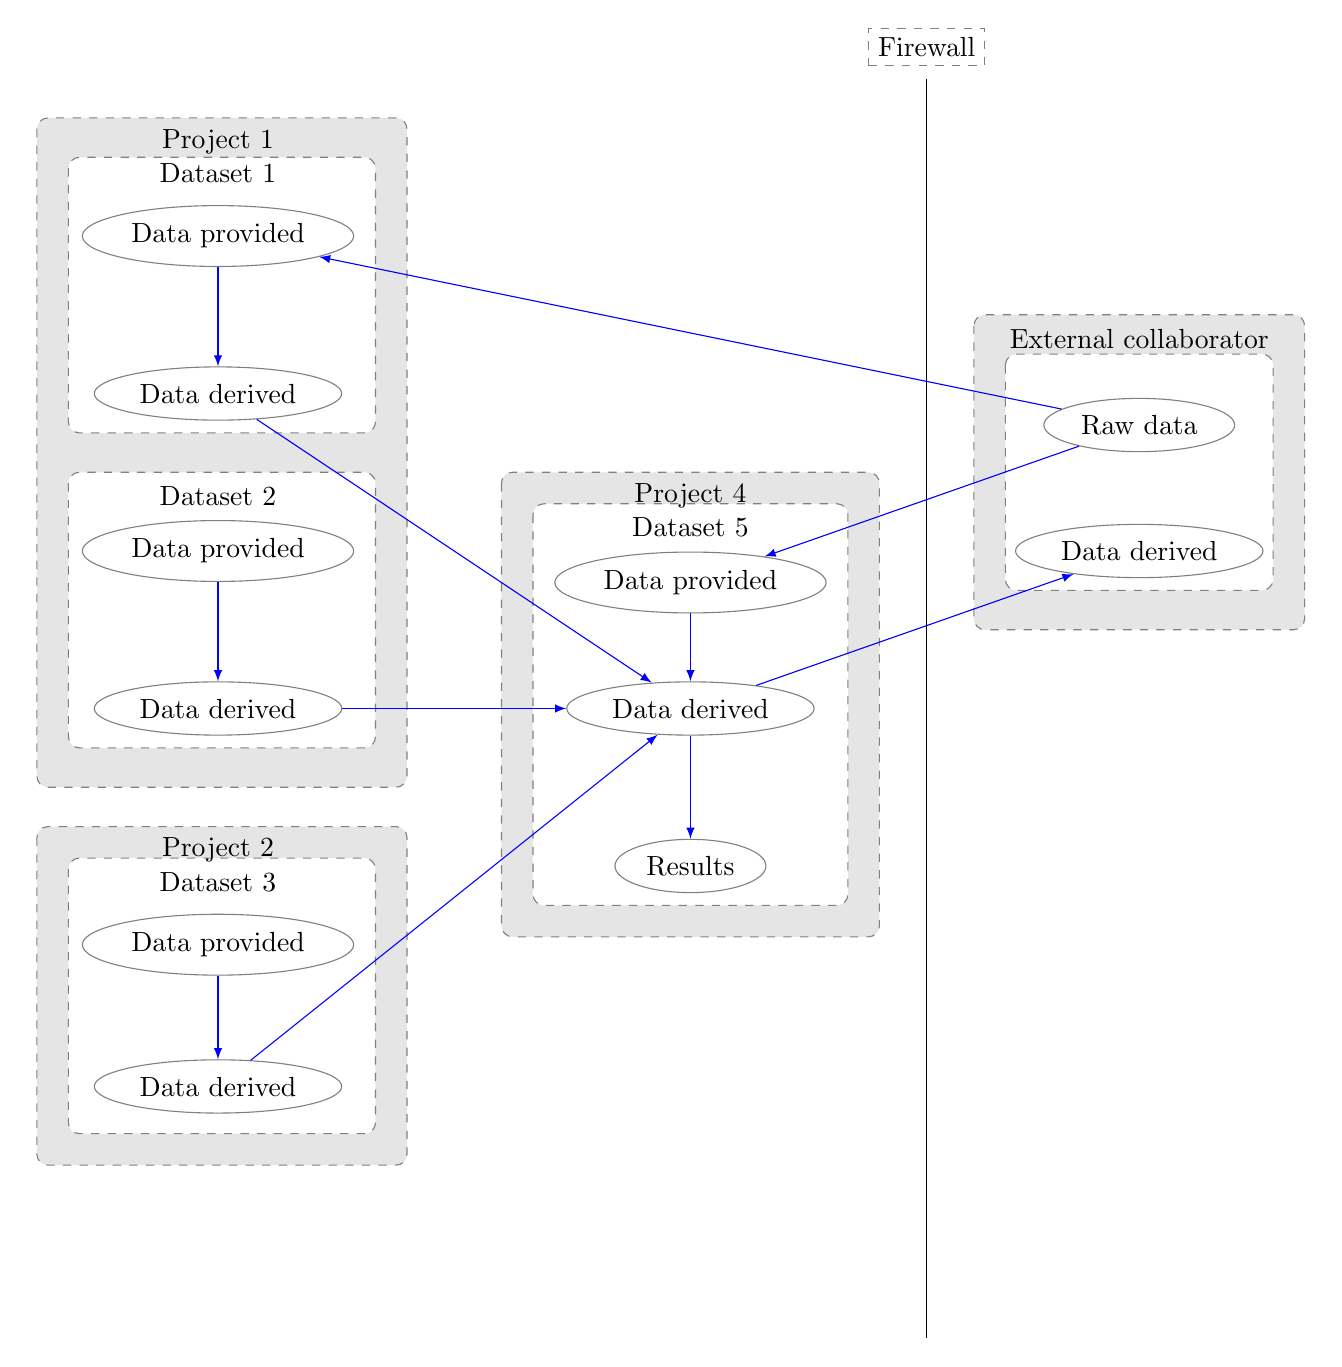
\begin{tikzpicture} [
            outpt/.style={->,blue!80!black,very thick},
            >=stealth,
         every node/.append style={align=center}]
%\tikzstyle{every node}=[draw,rectangle] 

%P1
\node (p1) at (0,1.2){Project 1};
\begin{pgfonlayer}{background}
   % Left-top corner of the background rectangle
   \path (-2.3,1.5) node (a13) {};
   % Right-bottom corner of the background rectanle
   \path (2.4, -7) node (c13) {};
   % Draw the background
   \path[fill=gray!20, rounded corners, draw=black!50, dashed]
   (a13) rectangle (c13);
\end{pgfonlayer}

%D1
\node (d1) at (0,.8) {Dataset 1};
\node (root) at (0,0) [draw=black!50,ellipse] {Data provided};
\node (GH) at (0,-2) [draw=black!50,ellipse]{Data derived}; 
\draw [-latex,color=blue] (root) -- (GH);
\begin{pgfonlayer}{background}
   % Left-top corner of the background rectangle
   \path (-1.9,1) node (a1) {};
   % Right-bottom corner of the background rectanle
   \path (2, -2.5) node (c1) {};
   % Draw the background
   \path[fill = white, rounded corners, draw=black!50, dashed]
   (a1) rectangle (c1);
\end{pgfonlayer}

%D2
\node (d2) at (0,-3.3) {Dataset 2};
\node (root1) at (0,-4) [draw=black!50,ellipse] {Data provided};
\node (GH1)   at (0,-6) [draw=black!50,ellipse]{Data derived}; 
\draw [-latex,color=blue] (root1) -- (GH1);
\begin{pgfonlayer}{background}
   % Left-top corner of the background rectangle
   \path (-1.9,-3) node (a12) {};
   % Right-bottom corner of the background rectanle
   \path (2, -6.5) node (c12) {};
   % Draw the background
   \path[fill = white, rounded corners, draw=black!50, dashed]
   (a12) rectangle (c12);
\end{pgfonlayer}



%P4
\node (p4) at (6, -3.3) {Project 4};
\begin{pgfonlayer}{background}
   % Left-top corner of the background rectangle
   \path (3.6,-3) node (a1p4) {};
   % Right-bottom corner of the background rectanle
   \path (8.4, -8.9) node (c1p4) {};
   % Draw the background
   \path[fill=gray!20, rounded corners, draw=black!50, dashed]
   (a1p4) rectangle (c1p4);
\end{pgfonlayer}

%D5
\node (p4) at (6, -3.7) {Dataset 5};
\node (local2) at (6,-4.4) [draw=black!50,ellipse]{Data provided};
\node (local) at (6,-6) [draw=black!50,ellipse]{Data derived};
\node (validated) at (6,-8) [draw=black!50,ellipse] {Results};  
\draw [-latex,color=blue] (GH) -- (local);
\draw [-latex,color=blue] (local) -- (validated);
\draw [-latex,color=blue] (local2) -- (local);
\draw [-latex,color=blue] (GH1) -- (local);

\begin{pgfonlayer}{background}
   % Left-top corner of the background rectangle
   \path (4,-3.4) node (a11) {};
   % Right-bottom corner of the background rectanle
   \path (8, -8.5) node (c11) {};
   % Draw the background
   \path[fill = white, rounded corners, draw=black!50, dashed]
   (a11) rectangle (c11);
\end{pgfonlayer}


%P2
\node (p2) at (0,-7.8) {Project 2};
\begin{pgfonlayer}{background}
   % Left-top corner of the background rectangle
   \path (-2.3,-7.5) node (a1p2) {};
   % Right-bottom corner of the background rectanle
   \path (2.4, -11.8) node (c1p2) {};
   % Draw the background
   \path[fill=gray!20, rounded corners, draw=black!50, dashed]
   (a1p2) rectangle (c1p2);
\end{pgfonlayer}


%D3
\node (d3) at (0,-8.2) {Dataset 3};
\node (local3) at (0,-9) [draw=black!50,ellipse]{Data provided};
\node (local31) at (0,-10.8) [draw=black!50,ellipse]{Data derived};
\draw [-latex,color=blue] (local3) -- (local31);
\draw [-latex,color=blue] (local31) -- (local);

\begin{pgfonlayer}{background}
   % Left-top corner of the background rectangle
   \path (-1.9,-7.9) node (a1d3) {};
   % Right-bottom corner of the background rectanle
   \path (2, -11.4) node (c1d3) {};
   % Draw the background
   \path[fill = white, rounded corners, draw=black!50, dashed]
   (a1d3) rectangle (c1d3);
\end{pgfonlayer}




% firewall
\node (firewall) at (9,2.4) [draw=black!50,dashed,rectangle]{Firewall}; 
\draw[](9, 2)--(9,-14);

%ext
\node (ext) at (11.7, -1.3) {External collaborator};
\begin{pgfonlayer}{background}
   % Left-top corner of the background rectangle
   \path (9.6,-1) node (a1ext) {};
   % Right-bottom corner of the background rectanle
   \path (13.8, -5) node (c1ext) {};
   % Draw the background
   \path[fill=gray!20, rounded corners, draw=black!50, dashed]
   (a1ext) rectangle (c1ext);
\end{pgfonlayer}

%extD
\node (local21) at (11.7,-2.4) [draw=black!50,ellipse]{Raw data};
\node (local31) at (11.7,-4) [draw=black!50,ellipse]{Data derived};

\draw [-latex,color=blue] (local21) -- (local2);
\draw [-latex,color=blue] (local) -- (local31);
\draw [-latex,color=blue] (local21) -- (root);

\begin{pgfonlayer}{background}
   % Left-top corner of the background rectangle
 \path (10,-1.5) node (a1ext2) {};
   % Right-bottom 5orner of the background rectanle
 \path (13.4, -4.5) node (c1ext2) {};
   % Draw the background
  \path[fill = white, rounded corners, draw=black!50, dashed]
  (a1ext2) rectangle (c1ext2);
\end{pgfonlayer}


%node (AP) at (-1,-3.5) [draw=black!50,ellipse]{Air pollution}
%node (ref) at (-0.5,-7) [draw=black!50,ellipse]{References \\(satellite, news, etc)}
%\tikzstyle{every node}=[] 



% .. controls +(0,-1) .. node (w2p)[near end,below left,color=black] {Data are read\\from source} (local);
%\draw [-latex,color=blue] (AP) .. controls +(.5,-1) .. node (w2p)[near end,above right,color=black] {Impute,\\ quantiles} (local);
%\draw [-latex,color=blue] (ref) .. controls +(0,1) .. node (w2p)[near end,above right,color=black] {Review} (local);

% .. controls +(.5,-1) .. node (w2p)[near end,above right,color=black] {Data entry of references\\+ events} (validated);

\end{tikzpicture} 

%\end{document}

\begin{tikzpicture} [
            outpt/.style={->,blue!80!black,very thick},
            >=stealth,
         every node/.append style={align=center}]
%\tikzstyle{every node}=[draw,rectangle] 

%P1
\node (p1) at (0,1.2){Project 1};
\begin{pgfonlayer}{background}
   % Left-top corner of the background rectangle
   \path (-2.3,1.5) node (a13) {};
   % Right-bottom corner of the background rectanle
   \path (2.4, -7) node (c13) {};
   % Draw the background
   \path[fill=gray!20, rounded corners, draw=black!50, dashed]
   (a13) rectangle (c13);
\end{pgfonlayer}

%D1
\node (d1) at (0,.8) {Dataset 1};
\node (root) at (0,0) [draw=black!50,ellipse] {Data provided};
\node (GH) at (0,-2) [draw=black!50,ellipse]{Data derived}; 
\draw [-latex,color=blue] (root) -- (GH);
\begin{pgfonlayer}{background}
   % Left-top corner of the background rectangle
   \path (-1.9,1) node (a1) {};
   % Right-bottom corner of the background rectanle
   \path (2, -2.5) node (c1) {};
   % Draw the background
   \path[fill = white, rounded corners, draw=black!50, dashed]
   (a1) rectangle (c1);
\end{pgfonlayer}

%D2
\node (d2) at (0,-3.3) {Dataset 2};
\node (root1) at (0,-4) [draw=black!50,ellipse] {Data provided};
\node (GH1)   at (0,-6) [draw=black!50,ellipse]{Data derived}; 
\draw [-latex,color=blue] (root1) -- (GH1);
\begin{pgfonlayer}{background}
   % Left-top corner of the background rectangle
   \path (-1.9,-3) node (a12) {};
   % Right-bottom corner of the background rectanle
   \path (2, -6.5) node (c12) {};
   % Draw the background
   \path[fill = white, rounded corners, draw=black!50, dashed]
   (a12) rectangle (c12);
\end{pgfonlayer}



%P4
\node (p4) at (6, -3.3) {Project 4};
\begin{pgfonlayer}{background}
   % Left-top corner of the background rectangle
   \path (3.6,-3) node (a1p4) {};
   % Right-bottom corner of the background rectanle
   \path (8.4, -8.9) node (c1p4) {};
   % Draw the background
   \path[fill=gray!20, rounded corners, draw=black!50, dashed]
   (a1p4) rectangle (c1p4);
\end{pgfonlayer}

%D5
\node (p4) at (6, -3.7) {Dataset 5};
\node (local2) at (6,-4.4) [draw=black!50,ellipse]{Data provided};
\node (local) at (6,-6) [draw=black!50,ellipse]{Data derived};
\node (validated) at (6,-8) [draw=black!50,ellipse] {Results};  
\draw [-latex,color=blue] (GH) -- (local);
%\draw [-latex,color=blue] (local) -- (validated);
\draw [-latex,color=blue] (local2) -- (local);
\draw [-latex,color=blue] (GH1) -- (local);

\begin{pgfonlayer}{background}
   % Left-top corner of the background rectangle
   \path (4,-3.4) node (a11) {};
   % Right-bottom corner of the background rectanle
   \path (8, -8.5) node (c11) {};
   % Draw the background
   \path[fill = white, rounded corners, draw=black!50, dashed]
   (a11) rectangle (c11);
\end{pgfonlayer}


%P2
\node (p2) at (0,-7.8) {Project 2};
\begin{pgfonlayer}{background}
   % Left-top corner of the background rectangle
   \path (-2.3,-7.5) node (a1p2) {};
   % Right-bottom corner of the background rectanle
   \path (2.4, -11.8) node (c1p2) {};
   % Draw the background
   \path[fill=gray!20, rounded corners, draw=black!50, dashed]
   (a1p2) rectangle (c1p2);
\end{pgfonlayer}


%D3
\node (d3) at (0,-8.2) {Dataset 3};
\node (local3) at (0,-9) [draw=black!50,ellipse]{Data provided};
\node (local31) at (0,-10.8) [draw=black!50,ellipse]{Data derived};
\draw [-latex,color=blue] (local3) -- (local31);
\draw [-latex,color=blue] (local31) -- (local);

\begin{pgfonlayer}{background}
   % Left-top corner of the background rectangle
   \path (-1.9,-7.9) node (a1d3) {};
   % Right-bottom corner of the background rectanle
   \path (2, -11.4) node (c1d3) {};
   % Draw the background
   \path[fill = white, rounded corners, draw=black!50, dashed]
   (a1d3) rectangle (c1d3);
\end{pgfonlayer}




% firewall
\node (firewall) at (9,2.4) [draw=black!50,dashed,rectangle]{Firewall}; 
\draw[](9, 2)--(9,-14);

%ext
\node (ext) at (11.7, -1.3) {External collaborator};
\begin{pgfonlayer}{background}
   % Left-top corner of the background rectangle
   \path (9.6,-1) node (a1ext) {};
   % Right-bottom corner of the background rectanle
   \path (13.8, -5) node (c1ext) {};
   % Draw the background
   \path[fill=gray!20, rounded corners, draw=black!50, dashed]
   (a1ext) rectangle (c1ext);
\end{pgfonlayer}

%extD
\node (local21) at (11.7,-2.4) [draw=black!50,ellipse]{Raw data};
\node (local31) at (11.7,-4) [draw=black!50,ellipse]{Data derived};

\draw [-latex,color=blue] (local21) -- (local2);
\draw [-latex,color=blue] (local) -- (local31);
%\draw [-latex,color=blue] (local21) -- (root);

\begin{pgfonlayer}{background}
   % Left-top corner of the background rectangle
 \path (10,-1.5) node (a1ext2) {};
   % Right-bottom 5orner of the background rectanle
 \path (13.4, -4.5) node (c12ext2) {};
   % Draw the background
  \path[fill = white, rounded corners, draw=black!50, dashed]
  (a1ext2) rectangle (c1ext2);
\end{pgfonlayer}

%savm
\node (ext) at (11.7, -7.8) {Secure Analysis VM};
\begin{pgfonlayer}{background}
   % Left-top corner of the background rectangle
   \path (9.6,-7.5) node (a1savm) {};
   % Right-bottom corner of the background rectanle
   \path (13.8, -11.8) node (c1savm) {};
   % Draw the background
   \path[fill=gray!20, rounded corners, draw=black!50, dashed]
   (a1savm) rectangle (c1savm);
\end{pgfonlayer}

%savmD
\node (savm1) at (11.7,-9) [draw=black!50,ellipse]{Data analysis};
\node (savm2) at (11.7,-10.8) [draw=black!50,ellipse]{Results};

\draw [-latex,color=blue] (local) -- (savm1);
\draw [-latex,color=blue] (savm1) -- (savm2);
\draw [-latex,color=blue] (savm2) -- (validated);

\begin{pgfonlayer}{background}
   % Left-top corner of the background rectangle
 \path (10,-7.9) node (a1savm2) {};
   % Right-bottom 5orner of the background rectanle
 \path (13.4, -11.4) node (c1savm2) {};
   % Draw the background
  \path[fill = white, rounded corners, draw=black!50, dashed]
  (a1savm2) rectangle (c1savm2);
\end{pgfonlayer}


%node (AP) at (-1,-3.5) [draw=black!50,ellipse]{Air pollution}
%node (ref) at (-0.5,-7) [draw=black!50,ellipse]{References \\(satellite, news, etc)}
%\tikzstyle{every node}=[] 



% .. controls +(0,-1) .. node (w2p)[near end,below left,color=black] {Data are read\\from source} (local);
%\draw [-latex,color=blue] (AP) .. controls +(.5,-1) .. node (w2p)[near end,above right,color=black] {Impute,\\ quantiles} (local);
%\draw [-latex,color=blue] (ref) .. controls +(0,1) .. node (w2p)[near end,above right,color=black] {Review} (local);

% .. controls +(.5,-1) .. node (w2p)[near end,above right,color=black] {Data entry of references\\+ events} (validated);

\end{tikzpicture} 

\end{document}
